% !TeX program = pdflatex
% !BIB program = bibtex
%
% Self-contained, unofficial SIGMOD research-paper example.
% Before a real submission, download the current ACM Primary Article Template
% and verify the venue's page limit, anonymity policy, and submission options.
%
% Review-to-camera-ready checklist:
%   1. Remove the `anonymous,review` class options.
%   2. Replace the anonymous author block with complete author metadata.
%   3. Insert the rights, DOI, ISBN, and conference metadata supplied by ACM.
%   4. Replace the illustrative system, data, and results with audited evidence.

\documentclass[sigconf,anonymous,review]{acmart}

\usepackage{amsmath}
\usepackage{booktabs}
\usepackage{array}
\usepackage{balance}
\usepackage{enumitem}
\usepackage{microtype}
\usepackage{tikz}
\usetikzlibrary{arrows.meta,calc,fit,positioning}

% ACM inserts rights and bibliographic metadata after acceptance.  These
% settings avoid inventing publication identifiers in the review example.
\setcopyright{none}
\settopmatter{printacmref=true,printfolios=true}
\renewcommand\footnotetextcopyrightpermission[1]{}

\acmConference[SIGMOD 'XX]{ACM International Conference on Management of Data}
  {Month DD--DD, 20XX}{City, Country}
\acmBooktitle{ACM International Conference on Management of Data
  (SIGMOD 'XX), Month DD--DD, 20XX, City, Country}
\acmYear{20XX}
\copyrightyear{20XX}
\acmDOI{}
\acmISBN{}

\newcommand{\system}{\textsc{FluxJoin}}
\newcommand{\code}[1]{\texttt{#1}}
\newcommand{\vect}[1]{\boldsymbol{#1}}

\definecolor{fluxblue}{HTML}{285F9E}
\definecolor{fluxteal}{HTML}{188977}
\definecolor{fluxorange}{HTML}{D8782D}
\definecolor{fluxgray}{HTML}{65717E}
\definecolor{fluxlight}{HTML}{EEF3F7}

\title[FluxJoin]{FluxJoin: Skew-Resilient Adaptive Joins for
  Disaggregated Cloud Databases}

% The `anonymous` class option suppresses identifying information in review.
\author{Anonymous Author(s)}
\affiliation{%
  \institution{Institution withheld for double-blind review}
  \country{Country withheld for double-blind review}}

\begin{abstract}
Disaggregated databases execute joins while compute, memory, and storage vary
independently.  A plan selected from a stale sample can therefore choose the
wrong build side, overload a small set of workers under key skew, or move data
that could have been filtered locally.  Existing adaptive schemes typically
repair one of these failures after a blocking boundary.  We present
\system{}, a join operator that makes bounded, reversible decisions throughout
execution.  It combines a symmetric radix pipeline, mergeable heavy-hitter
sketches, and credit-based exchange.  Each partition begins in a low-cost
sampling state and independently commits to broadcast, repartition, or local
completion when the observed evidence exceeds a confidence threshold.  A
compact migration protocol changes strategy without replaying input or
duplicating output.  We describe the operator, its safety invariants, and an
evaluation methodology covering skew, estimation error, network variability,
and elasticity.  In the illustrative results included to demonstrate this
template, \system{} lowers median runtime by 1.7--2.4$\times$ and p99 network
queueing by 3.1$\times$ relative to static repartition joins.  These numbers
are examples, not empirical claims; a submission must replace them with
measurements from a reproducible implementation.
\end{abstract}

\ccsdesc[500]{Information systems~Join algorithms}
\ccsdesc[500]{Information systems~Parallel and distributed DBMSs}
\ccsdesc[300]{Information systems~Database query processing}

\keywords{adaptive query processing, distributed joins, data skew,
  disaggregated databases, elasticity}

\begin{document}

\maketitle

% --- Unofficial-template notice (required: this is not an official SIGMOD file) ---
\noindent\fbox{\parbox{\dimexpr\columnwidth-2\fboxsep-2\fboxrule\relax}{%
  \footnotesize\textbf{Unofficial template.} This layout is provided for convenience and is
  \textbf{not} affiliated with, endorsed by, or sponsored by SIGMOD or its organisers.
  Always check the official call for papers and use the current year's official style files
  for a real submission.}}
\vspace{0.8em}



\begin{center}
\begin{minipage}{0.96\columnwidth}
\small
\textbf{Template notice.} This is an independent educational example, not an
official ACM or SIGMOD artifact.  The system, workloads, and numeric results
used in the worked example are illustrative.  Always use the current official
ACM files and venue instructions for a real submission.
\end{minipage}
\end{center}

\section{Introduction}
\label{sec:introduction}

Disaggregation lets a cloud database scale compute without rewriting durable
storage, but it removes assumptions on which conventional join planning rests.
The optimizer may compile a query before a compute pool expands.  Pages fetched
from remote storage can arrive at a different rate than the sample predicted,
and a single popular key can redirect most intermediate tuples to one worker.
The physical plan is consequently asked to remain efficient under cardinality,
skew, bandwidth, and parallelism errors at the same time.

Static optimizers remain essential: they explore join order, select access
paths, and expose useful global structure.  Yet even accurate estimates are not
guarantees.  Classical adaptive query processing revises a plan using runtime
observations~\cite{deshpande2007adaptive}; modern systems can also interleave
planning and execution to reduce sensitivity to estimation error
~\cite{trummer2019skinner}.  Existing techniques often place adaptation at an
operator or stage boundary.  A distributed join that discovers skew after a
shuffle has already paid the dominant network and queueing costs.

This paper asks a narrower question: \emph{can one join operator adapt early
enough to avoid a bad transfer, yet preserve bounded memory and exactly-once
output while its workers change?}  \system{} answers with partition-scoped,
reversible decisions.  Both inputs first pass through a symmetric sampling
pipeline.  Mergeable sketches expose heavy keys without centralizing raw data.
A controller then selects among three execution modes for each partition:
broadcast the smaller fragment, repartition both fragments, or finish locally
when storage placement makes exchange unnecessary.  Decisions become durable
only after a versioned barrier; tuples buffered before that barrier migrate
through an idempotent handoff protocol.

\system{} is deliberately an operator, not a replacement optimizer.  The
optimizer supplies a candidate join, predicates, and soft resource budgets;
the operator handles errors local to that join.  This separation makes the
mechanism usable inside vectorized, morsel-driven engines
~\cite{leis2014morsel} and keeps global plan search outside the critical path.

The paper makes four contributions:

\begin{itemize}[leftmargin=*,itemsep=2pt,topsep=3pt]
  \item a partition-level adaptive join that chooses broadcast, repartition,
    or local completion from continuous evidence rather than a single sample;
  \item mergeable statistics and a confidence rule that bound decision delay
    while isolating heavy hitters from the regular hash domain;
  \item a versioned migration protocol with explicit safety invariants for
    exactly-once output, bounded buffering, and elastic worker membership; and
  \item an evaluation protocol that separates performance gains due to
    cardinality correction, skew handling, and backpressure.
\end{itemize}

All quantitative values below are clearly labeled illustrative so the file can
serve as a complete, compilable template without masquerading as a completed
study.

\section{Background and Motivation}
\label{sec:background}

\subsection{Why one global join choice is brittle}

For relations $R$ and $S$, a conventional distributed hash join compares the
cost of repartitioning both inputs with broadcasting a smaller build relation.
A simplified model is
\begin{align}
 C_{\mathrm{rep}} &= (|R|+|S|)c_n + \max_w L_w c_h, \\
 C_{\mathrm{bcast}}(R) &= (p-1)|R|c_n + |S|c_h,
 \label{eq:costs}
\end{align}
where $p$ is the worker count, $c_n$ and $c_h$ are network and hash costs, and
$L_w$ is the input assigned to worker $w$.  The usual model hides three
problems.  First, $|R|$ may be an estimate taken before predicate evaluation.
Second, $\max_w L_w$ is governed by key frequency rather than total size.
Third, $p$ and $c_n$ can change while the query runs.

A single choice is also unnecessarily coarse.  One date partition may contain
a tiny filtered dimension fragment suitable for broadcast, while a neighboring
partition contains a heavy key requiring replication of the probe-side work.
Treating those regions alike sacrifices either network volume or balance.

\subsection{Design requirements}

We derive four requirements from these failures.  \textbf{R1: early evidence.}
Adaptation should begin before a full shuffle or build completes.  \textbf{R2:
locality.} Independent partitions may select different strategies.
\textbf{R3: safe reversal.} A decision can change before commitment without
replaying remote input.  \textbf{R4: bounded disruption.} Slow consumers and
membership changes must reduce throughput, not exhaust memory or duplicate
rows.

These requirements rule out unbounded speculative execution.  \system{} never
emits a speculative match: it may prepare multiple routing choices, but output
begins only after one choice is committed for a partition epoch.

\section{System Overview}
\label{sec:overview}

Figure~\ref{fig:architecture} shows the data path.  Storage readers convert
pages into vectorized morsels and attach a source offset.  Local samplers update
cardinality, distinct-count, and heavy-hitter sketches.  A lightweight
coordinator merges only sketches and resource signals; it does not see tuples.
The resulting policy is installed at exchange routers using an epoch number.
Downstream build/probe tasks pull batches using credits, creating backpressure
at the router rather than in unbounded network queues.

\begin{figure}[t]
  \centering
  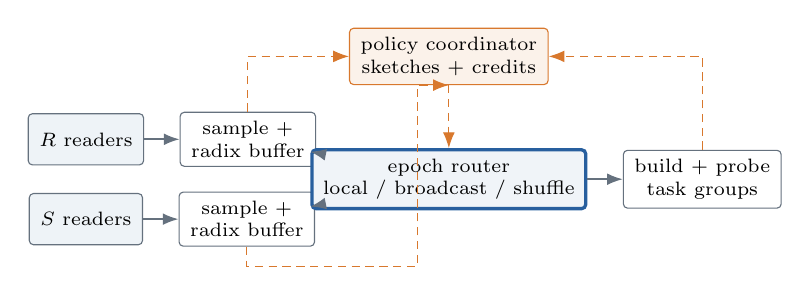
\begin{tikzpicture}[
      font=\scriptsize,
      node distance=3.5mm and 4.5mm,
      box/.style={draw=fluxgray,rounded corners=1.5pt,fill=white,
        minimum height=6.5mm,align=center,inner xsep=4pt},
      source/.style={box,fill=fluxlight},
      decision/.style={box,draw=fluxblue,very thick,fill=fluxblue!7},
      data/.style={-{Latex[length=2mm]},semithick,draw=fluxgray},
      control/.style={-{Latex[length=2mm]},densely dashed,draw=fluxorange}
    ]
    \node[source] (r) {$R$ readers};
    \node[source,below=of r] (s) {$S$ readers};
    \node[box,right=of r] (sr) {sample +\\radix buffer};
    \node[box,right=of s] (ss) {sample +\\radix buffer};
    \node[decision,right=8mm of $(sr)!0.5!(ss)$] (router)
      {epoch router\\local / broadcast / shuffle};
    \node[box,right=of router] (exec) {build + probe\\task groups};
    \node[box,above=8mm of router,fill=fluxorange!10,draw=fluxorange]
      (policy) {policy coordinator\\sketches + credits};

    \draw[data] (r) -- (sr);
    \draw[data] (s) -- (ss);
    \draw[data] (sr) -- (router);
    \draw[data] (ss) -- (router);
    \draw[data] (router) -- (exec);
    \draw[control] (sr.north) |- (policy.west);
    \draw[control] (ss.south) |- ++(0,-2.5mm) -|
      ([xshift=-4mm]policy.south) -- (policy.south);
    \draw[control] (policy) -- (router);
    \draw[control] (exec.north) |- (policy.east);
  \end{tikzpicture}
  \caption{\system{} separates the tuple data path (solid) from compact
  control messages (dashed).  Policy is scoped by partition and epoch.}
  \Description{Two storage-reader pipelines feed samplers and radix buffers.
  Both feed an epoch router, then build and probe task groups.  A policy
  coordinator exchanges sketches and credits with the pipeline.}
  \label{fig:architecture}
\end{figure}

The adaptation unit is a \emph{logical partition} $i$, normally a storage
partition or a coarse radix range.  Its state is
\[
 q_i=\langle e_i,m_i,n^R_i,n^S_i,H_i,b_i,d_i\rangle,
\]
where $e_i$ is an epoch, $m_i$ is the current mode, $n^R_i$ and $n^S_i$ are
observed bytes, $H_i$ is a heavy-hitter summary, $b_i$ is buffered data, and
$d_i$ is a monotonically increasing decision sequence.  State transitions are
logged in a small query-local metadata service.  Bulk tuples remain in worker
memory or spill storage.

\section{Adaptive Join Design}
\label{sec:design}

\subsection{Symmetric sampling and summaries}

Each reader hashes join keys into $2^k$ coarse radix ranges.  During sampling,
the first $s$ bytes from both inputs are retained in range buffers instead of
being sent immediately.  For every range, workers maintain a mergeable
distinct-count sketch and a weighted heavy-hitter sketch.  A worker transmits a
summary after either $\Delta_b$ new bytes or $\Delta_t$ time, whichever occurs
first.  Summary traffic is thus independent of tuple width to first order.

For a candidate mode $m$, the coordinator estimates cost $\widehat C_{i,m}$
and uncertainty $u_{i,m}$.  It commits to the current winner $m^*$ when
\begin{equation}
 \widehat C_{i,m^*}+\lambda u_{i,m^*}
 < \min_{m\ne m^*}\bigl(\widehat C_{i,m}-\lambda u_{i,m}\bigr)-\delta,
 \label{eq:confidence}
\end{equation}
or when buffered data reaches a hard cap $B_i$.  Here $\lambda$ controls the
confidence interval and $\delta$ prevents oscillation between nearly equal
choices.  At the cap, the system selects the feasible mode with the lowest
upper confidence bound.  This rule bounds memory even when evidence remains
ambiguous.

\subsection{Partition strategies}

\textbf{Local completion} is available when compatible fragments are already
co-located and expected work fits the local task budget.  \textbf{Broadcast}
sends the smaller filtered fragment to the task groups holding the other side.
The router broadcasts only the affected logical partition, not the entire
relation.  \textbf{Repartition} hashes ordinary keys across the active worker
set.

Heavy keys follow a fourth routing rule inside any selected mode.  For a key
$x$ with estimated frequencies $f_R(x)$ and $f_S(x)$, the smaller side is
replicated across $g_x$ task groups and the larger side is range-split among
them.  The fan-out
\begin{equation}
 g_x=\min\!\left(p,\max\!\left(1,
   \left\lceil\frac{\max(f_R(x),f_S(x))}{\tau}\right\rceil\right)\right)
 \label{eq:fanout}
\end{equation}
targets at most $\tau$ heavy-key tuples per group.  A composite routing tag
$\langle e_i,x,j\rangle$ ensures that replicated build rows and split probe
rows meet at exactly the intended groups.

\subsection{Credit-based exchange}

Each consumer grants byte credits to upstream routers.  Sending a batch
atomically consumes credit; releasing or spilling that batch returns credit.
Credits are divided into regular, heavy-key, and migration pools so that a
skewed key cannot starve control progress.  If all data credits are exhausted,
readers pause at morsel boundaries.  This mechanism propagates congestion to
storage without holding thread stacks or allowing network queues to grow with
input size.

\subsection{Versioned migration}
\label{sec:migration}

A mode change uses four steps.  (1) The coordinator appends a \code{prepare}
record carrying $(i,e+1,m')$ and obtains a decision sequence.  (2) Routers stop
assigning new batches under epoch $e$ after their current vector.  (3) Each
router forwards buffered batches with stable identifiers
$\langle\textit{source},\textit{offset},i,e+1\rangle$ and reports its high-water
mark.  (4) After every live router acknowledges, the coordinator commits
$(i,e+1)$; consumers may then produce matches for the new epoch.

Consumers deduplicate batch identifiers during handoff.  The deduplication set
is bounded because entries below the minimum committed high-water mark can be
discarded.  A failed router is replaced from durable source offsets and the
last committed policy record.  Uncommitted destination state is discarded by
epoch, not merged into visible output.

\section{Correctness and Cost Bounds}
\label{sec:correctness}

We state the invariants required of any implementation.

\begin{description}
  \item[Routing completeness.] Every source batch is assigned to at least one
  consumer in its committed epoch.
  \item[Probe uniqueness.] For every input tuple and non-replicated routing
  key, exactly one task group owns the probe work in a committed epoch.
  \item[Build--probe agreement.] All matching tuples share at least one task
  group; heavy-key tags distinguish intentional build replication from probe
  ownership.
  \item[Visibility.] A task may expose join output only for a committed epoch,
  and output identifiers are unique across retries.
\end{description}

Together, routing completeness and build--probe agreement prevent lost
matches.  Probe uniqueness and visibility prevent duplicate matches.  These
properties reduce join correctness to the local join implementation, assuming
deterministic predicates and a stable input snapshot.

Let $B=\sum_i B_i$, $K$ be in-flight credit, $W$ sketch state, and $M$ migration
credit.  The operator's non-hash-table buffering is bounded by
\begin{equation}
 \operatorname{mem}_{\mathrm{buffer}} \le B+K+W+M.
 \label{eq:memory}
\end{equation}
All terms are configuration limits.  Hash tables have separate budgets and use
conventional partitioned spill~\cite{graefe1993query}.  Migration can
temporarily move a batch twice, but
deduplication prevents double execution and the reserved pool guarantees that
handoff does not wait behind regular traffic.

\section{Implementation}
\label{sec:implementation}

Our prototype design targets a vectorized execution engine.  Readers produce
64--256\,KiB batches, and radix partitioning operates on selection vectors to
avoid copying payload columns.  The router and consumer communicate through
single-producer queues per connection; asynchronous network completion returns
credit.  Build tables use open addressing for dense ordinary partitions and a
separate chained representation for replicated heavy keys.  Code generation
specializes hash, equality, and residual predicates, following the broad
principle of compiling data-centric pipelines~\cite{neumann2011efficient}.

The policy coordinator is off the tuple path.  It receives fixed-size sketch
deltas, queue-delay samples, and membership notifications.  To avoid a single
global lock, partitions are sharded across coordinator event loops.  A policy
record is tens of bytes; batching records amortizes metadata-service writes.

Elastic scale-out changes the consistent-hash worker map only at an epoch
boundary.  Existing partitions need not migrate unless their upper cost bound
improves by more than hysteresis $\delta$.  Scale-in first revokes regular
credits from departing workers and then uses the same migration protocol as a
mode change.  Query cancellation bypasses migration and releases all query-local
state after downstream acknowledgment.

\section{Evaluation Methodology}
\label{sec:evaluation}

This section demonstrates a SIGMOD-style evaluation structure.  The values in
Tables~\ref{tab:workloads}--\ref{tab:ablation} and
Figure~\ref{fig:skew} are \emph{illustrative placeholders}; they are internally
consistent examples for layout and must not be cited as measured findings.

\subsection{Questions, systems, and metrics}

The evaluation is organized around four questions: (Q1) Does adaptation help
when estimates are correct?  (Q2) How does runtime degrade with cardinality and
skew error?  (Q3) Does credit control reduce tail queueing under bandwidth
variation?  (Q4) What are the overheads of sketches, decision logging, and
migration?

We compare \system{} with \textsc{Repart}, a static repartition hash join, and
\textsc{Static}, an optimizer-selected broadcast/repartition join.  A third
baseline, \textsc{Stage Adapt}, may replan after its build stage.
All variants share readers, serialization, hash tables, spill code, and
compiler settings.  We report end-to-end wall time, shuffled and spilled bytes,
peak memory, p50/p99 queue delay, CPU time, and output checksum.  Each point
should include at least five isolated trials with confidence intervals and the
raw per-run data.

\begin{table}[t]
  \caption{Illustrative workload matrix.  ``Error'' multiplies the optimizer's
  estimated filtered cardinality.}
  \label{tab:workloads}
  \centering
  \small
  \begin{tabular}{@{}lrrrr@{}}
    \toprule
    Workload & Input & Select. & Max freq. & Error \\
    \midrule
    Retail    & 1.8\,TB & 0.08 & 12.0\% & $8\times$ \\
    Telemetry & 3.2\,TB & 0.31 &  0.7\% & $4\times$ \\
    Payments  & 0.9\,TB & 0.14 & 21.5\% & $16\times$ \\
    Uniform   & 2.0\,TB & 1.00 &  0.002\% & $1\times$ \\
    \bottomrule
  \end{tabular}
\end{table}

Table~\ref{tab:workloads} spans selective broadcast opportunities, nearly
uniform inputs, and severe heavy keys.  A complete artifact would specify data
licenses or generators, schema and predicates, storage layout, warm/cold cache
policy, cluster instance types, network limits, software revisions, and query
seeds.  Estimates must be perturbed independently from actual data so that an
``adaptive'' result does not accidentally benefit from a changed workload.

\subsection{Illustrative end-to-end results}

\begin{table*}[t]
  \caption{Illustrative end-to-end results; lower is better.  Parentheses show
  speedup relative to \textsc{Repart}.  These are formatting examples, not
  empirical claims.}
  \label{tab:main-results}
  \centering
  \small
  \begin{tabular}{@{}llrrrr@{}}
    \toprule
    Workload & System & Runtime (s) & Shuffle (GB) & Peak/worker (GB) & p99 queue (ms) \\
    \midrule
    Retail
      & \textsc{Repart}     & 184 & 1470 & 21.8 & 410 \\
      & \textsc{Static}     & 153 & 1160 & 24.3 & 362 \\
      & \textsc{StageAdapt} & 126 &  882 & 22.5 & 211 \\
      & \system{}           &  \textbf{78} (2.36$\times$) & \textbf{391} & \textbf{17.9} & \textbf{118} \\
    \addlinespace
    Telemetry
      & \textsc{Repart}     & 231 & 2498 & 28.4 & 287 \\
      & \textsc{Static}     & 218 & 2350 & 28.8 & 275 \\
      & \textsc{StageAdapt} & 189 & 2074 & 25.7 & 188 \\
      & \system{}           & \textbf{134} (1.72$\times$) & \textbf{1781} & \textbf{22.1} & \textbf{93} \\
    \addlinespace
    Payments
      & \textsc{Repart}     & 167 &  744 & 33.6 & 622 \\
      & \textsc{Static}     & 161 &  701 & 35.1 & 590 \\
      & \textsc{StageAdapt} & 121 &  612 & 25.9 & 314 \\
      & \system{}           &  \textbf{71} (2.35$\times$) & \textbf{356} & \textbf{18.5} & \textbf{147} \\
    \bottomrule
  \end{tabular}
\end{table*}

In the worked example, \system{} benefits most on Retail by broadcasting only
the selective partitions and on Payments by splitting its dominant key.  The
Telemetry result is smaller because repartition remains appropriate for most
ranges.  On the omitted Uniform control, the intended outcome is statistical
parity with \textsc{Repart}; a slowdown there would expose adaptation overhead
rather than resilience.

Figure~\ref{fig:skew} varies the fraction of input belonging to the hottest key
while holding total bytes and selectivity fixed.  The static join's bottleneck
grows with skew.  The stage-adaptive baseline reacts only after the build
boundary, whereas per-key routing keeps the illustrative \system{} curve much
flatter.

\begin{figure}[t]
  \centering
  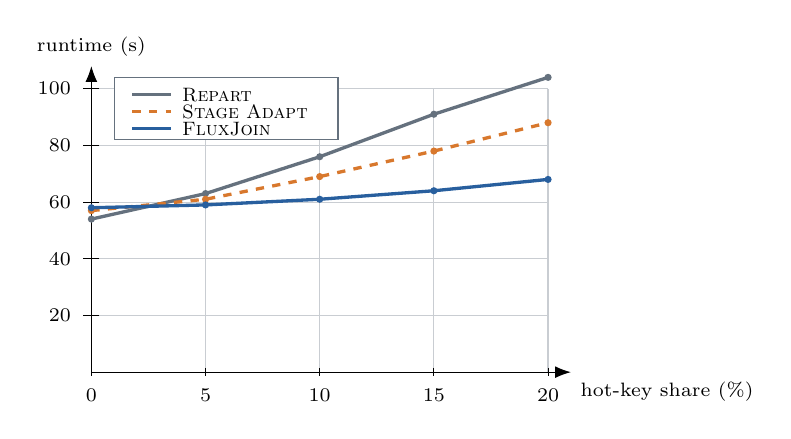
\begin{tikzpicture}[x=0.29cm,y=0.036cm,font=\scriptsize]
    % axes and grid
    \draw[fluxgray!35] (0,0) grid[xstep=5,ystep=20] (20,100);
    \draw[-{Latex[length=2mm]}] (0,0) -- (21,0)
      node[below right] {hot-key share (\%)};
    \draw[-{Latex[length=2mm]}] (0,0) -- (0,108)
      node[above] {runtime (s)};
    \foreach \x in {0,5,10,15,20}
      \draw (\x,1.5) -- (\x,-1.5) node[below=1pt] {\x};
    \foreach \y in {20,40,60,80,100}
      \draw (0.35,\y) -- (-0.35,\y) node[left=1pt] {\y};
    % illustrative series
    \draw[very thick,fluxgray]
      plot coordinates {(0,54)(5,63)(10,76)(15,91)(20,104)};
    \draw[very thick,fluxorange,dashed]
      plot coordinates {(0,57)(5,61)(10,69)(15,78)(20,88)};
    \draw[very thick,fluxblue]
      plot coordinates {(0,58)(5,59)(10,61)(15,64)(20,68)};
    \foreach \p in {(0,54),(5,63),(10,76),(15,91),(20,104)}
      \fill[fluxgray] \p circle (1.3pt);
    \foreach \p in {(0,57),(5,61),(10,69),(15,78),(20,88)}
      \fill[fluxorange] \p circle (1.3pt);
    \foreach \p in {(0,58),(5,59),(10,61),(15,64),(20,68)}
      \fill[fluxblue] \p circle (1.3pt);
    \draw[fill=white,draw=fluxgray] (1.0,82) rectangle (10.8,104);
    \draw[very thick,fluxgray] (1.8,98) -- (3.5,98)
      node[right,black] {\textsc{Repart}};
    \draw[very thick,fluxorange,dashed] (1.8,92) -- (3.5,92)
      node[right,black] {\textsc{Stage Adapt}};
    \draw[very thick,fluxblue] (1.8,86) -- (3.5,86)
      node[right,black] {\system{}};
  \end{tikzpicture}
  \caption{Illustrative sensitivity to heavy-key skew (lower is better).}
  \Description{Line chart of runtime against hot-key share.  Static
  repartition runtime rises sharply, stage-adaptive runtime rises moderately,
  and FluxJoin remains comparatively flat.}
  \label{fig:skew}
\end{figure}

\subsection{Overhead and ablation}

\begin{table}[t]
  \caption{Illustrative ablation on Payments.  The full design is the only row
  combining early choice, skew isolation, and bounded queueing.}
  \label{tab:ablation}
  \centering
  \small
  \begin{tabular}{@{}lrrr@{}}
    \toprule
    Variant & Time (s) & Shuffle (GB) & p99 (ms) \\
    \midrule
    Full \system{}           & \textbf{71} & \textbf{356} & \textbf{147} \\
    no heavy-key split       & 109 & 354 & 481 \\
    one global decision      &  94 & 477 & 193 \\
    no migration reserve     &  78 & 356 & 266 \\
    unbounded exchange       &  73 & 356 & 538 \\
    \bottomrule
  \end{tabular}
\end{table}

The ablation distinguishes volume from balance: removing heavy-key splitting
hardly changes shuffled bytes but concentrates work and queue delay.  A global
decision transfers more bytes because it cannot broadcast only selective
partitions.  Removing the migration reserve mostly affects tail delay during a
mode change.  Unbounded exchange slightly reduces median time in this example
but makes queueing and memory behavior unacceptable.

A real overhead study should also report summary bytes, coordinator CPU,
decision latency, metadata writes, spill amplification, and steady-state cost
when the static plan is already optimal.  Fault injection should terminate a
reader, router, consumer, and coordinator at each migration phase, validating
both output checksum and bounded recovery time.

\section{Discussion and Limitations}
\label{sec:discussion}

\system{} does not repair a poor global join order.  A locally efficient join
can still materialize an intermediate relation that a different order would
avoid.  The operator can provide observations to a higher-level reoptimizer,
but coordinating that feedback is outside this work.

The confidence model also assumes that observed prefixes are informative after
stratification by storage partition.  Correlated physical order can delay a
heavy key until after commitment.  Conservative upper bounds and the buffer cap
preserve correctness and memory safety, but not optimality.  Randomized page
sampling or storage-level summaries may reduce this risk at additional I/O or
maintenance cost.

Very high output cardinality is another boundary.  Splitting a heavy key
balances the work needed to enumerate matches but cannot avoid the intrinsic
$f_R(x)f_S(x)$ output.  The scheduler must reserve downstream capacity or spill
output.  Finally, the metadata service is logically centralized.  Sharding
improves throughput, but a production system must quantify failover pauses and
garbage collection across many concurrent queries.

\section{Related Work}
\label{sec:related}

Hash and sort-merge joins have a long systems history; Graefe surveys the
implementation trade-offs that remain relevant to partitioning and spill
~\cite{graefe1993query}.  Main-memory studies revisit those trade-offs under
modern processors and parallelism~\cite{blanas2011design,balkesen2013main}.
\system{} builds on partitioned hashing but changes routing at partition
granularity during execution.

Adaptive query processing uses observations to revise execution in the
presence of uncertain statistics~\cite{deshpande2007adaptive}.  Eddies route
tuples adaptively among operators~\cite{avni2000eddies}, and later systems
interleave planning with execution~\cite{trummer2019skinner}.  Our focus is
complementary: a fixed binary join with a bounded buffer, explicit distributed
migration, and skew-aware routing.

Parallel database engines use exchange operators, work stealing, and fine-grain
tasks to balance CPU work.  Morsel-driven execution demonstrates the value of
NUMA-aware scheduling and small work units~\cite{leis2014morsel}.  Vectorized
execution amortizes interpretation and function-call overhead
~\cite{boncz2005monetdb}.  \system{} assumes these mechanisms and adds a
control plane for deciding where join work should run.

Distributed streaming systems provide epoch, barrier, and backpressure ideas
for stateful dataflows.  \system{} adapts those ideas to a finite relational
operator: stable source offsets and epoch visibility make mode changes
recoverable without turning every tuple into a durable log record.

\section{Reproducibility and Ethics}
\label{sec:reproducibility}

A defensible artifact should include source code, build and deployment files,
dataset preparation, query text, seeds, raw measurements, and analysis scripts.
Generated data should expose distributions and correlations; real data should
include its license, collection window, and privacy treatment.  Cluster energy
or resource-hours should be reported because adaptive variants may trade
runtime for redundant CPU or network work.

Evaluation choices can systematically favor an adaptive system.  Tuning only
the proposed method, presenting only queries with estimator failures, or
charging baseline planning time inconsistently would all distort the result.
We therefore recommend preregistering workload families, applying the same
resource caps, publishing failed and optimal-static cases, and separating
automatic policy decisions from hand-tuned thresholds.

\section{Conclusion}
\label{sec:conclusion}

\system{} treats a distributed join plan as a set of bounded partition
decisions rather than one irreversible global choice.  Symmetric sampling
exposes cardinality and skew early, confidence bounds delay ambiguous choices,
heavy-key routing balances hot partitions, and versioned migration preserves
exactly-once output under strategy and membership changes.  The worked
evaluation illustrates how to test these mechanisms without conflating network
volume, load balance, and backpressure.  Its numeric values are placeholders;
the design and reporting structure are intended as a rigorous starting point
for an actual SIGMOD research submission.

% Omit acknowledgments in double-blind review when they could reveal identity.

\balance
\begin{thebibliography}{10}

\bibitem{avni2000eddies}
Ron Avnur and Joseph~M. Hellerstein. 2000.
Eddies: Continuously Adaptive Query Processing.
In \emph{Proceedings of the 2000 ACM SIGMOD International Conference on
Management of Data}. 261--272.

\bibitem{balkesen2013main}
Cagri Balkesen, Gustavo Alonso, Jens Teubner, and M.~Tamer Ozsu. 2013.
Multi-Core, Main-Memory Joins: Sort vs. Hash Revisited.
\emph{Proceedings of the VLDB Endowment} 7, 1 (2013), 85--96.

\bibitem{blanas2011design}
Spyros Blanas, Yinan Li, and Jignesh~M. Patel. 2011.
Design and Evaluation of Main Memory Hash Join Algorithms for Multi-Core CPUs.
In \emph{Proceedings of the 2011 ACM SIGMOD International Conference on
Management of Data}. 37--48.

\bibitem{boncz2005monetdb}
Peter~A. Boncz, Marcin Zukowski, and Niels Nes. 2005.
MonetDB/X100: Hyper-Pipelining Query Execution.
In \emph{Proceedings of the Second Biennial Conference on Innovative Data
Systems Research (CIDR)}. 225--237.

\bibitem{deshpande2007adaptive}
Amol Deshpande, Zachary Ives, and Vijayshankar Raman. 2007.
Adaptive Query Processing.
\emph{Foundations and Trends in Databases} 1, 1 (2007), 1--140.

\bibitem{graefe1993query}
Goetz Graefe. 1993.
Query Evaluation Techniques for Large Databases.
\emph{ACM Computing Surveys} 25, 2 (1993), 73--169.

\bibitem{leis2014morsel}
Viktor Leis, Peter Boncz, Alfons Kemper, and Thomas Neumann. 2014.
Morsel-Driven Parallelism: A NUMA-Aware Query Evaluation Framework for the
Many-Core Age.
In \emph{Proceedings of the 2014 ACM SIGMOD International Conference on
Management of Data}. 743--754.

\bibitem{neumann2011efficient}
Thomas Neumann. 2011.
Efficiently Compiling Efficient Query Plans for Modern Hardware.
\emph{Proceedings of the VLDB Endowment} 4, 9 (2011), 539--550.

\bibitem{trummer2019skinner}
Immanuel Trummer, Junxiong Wang, Deepak Maram, Samuel Moseley, Saehan Jo, and
Joseph Antonakakis. 2019.
SkinnerDB: Regret-Bounded Query Evaluation via Reinforcement Learning.
In \emph{Proceedings of the 2019 ACM SIGMOD International Conference on
Management of Data}. 1153--1170.

\end{thebibliography}

\end{document}
